% E8: v4 per Robin's spec.
% - Inputs arrow exits middle of inp.west.
% - Small refinement boxes right-aligned with main; |-> elbow arrow
%   from main.south_west into small.west.
% - Whole-body box moved down so the whole->SAR_wb arrow stays
%   strictly east-west (parallel to the others).
% - Inputs lowered; above it a small dashed "+ Corrections" box,
%   joined to the Formula box via a curved arrow.
\documentclass[tikz,border=2pt]{standalone}
\usepackage{tikz}
\usetikzlibrary{arrows.meta,positioning,calc,fit,backgrounds,bending}
\usepackage{amsmath,bm}
\definecolor{outA}{RGB}{216,234,251}
\definecolor{outB}{RGB}{251,234,216}
\definecolor{outC}{RGB}{226,247,217}
\newcommand{\Sinc}{S_{\mathrm{inc}}}
\newcommand{\Sab}{S_{\mathrm{ab}}}
\newcommand{\rr}{\mathbf{r}}
\newcommand{\khat}{\hat{\bm{k}}}
\newcommand{\nhat}{\hat{\bm{n}}}
\newcommand{\Tavg}{T_{\mathrm{avg}}}
\newcommand{\Tbar}{\bar{T}}
\newcommand{\Tlay}{T_{\mathrm{lay}}}
\newcommand{\Aab}{A_{\mathrm{ab}}}
\newcommand{\Vis}{V}
\newcommand{\SabAvg}{\langle S_{\mathrm{ab}}\rangle_{4\,\mathrm{cm}^2}}

\begin{document}
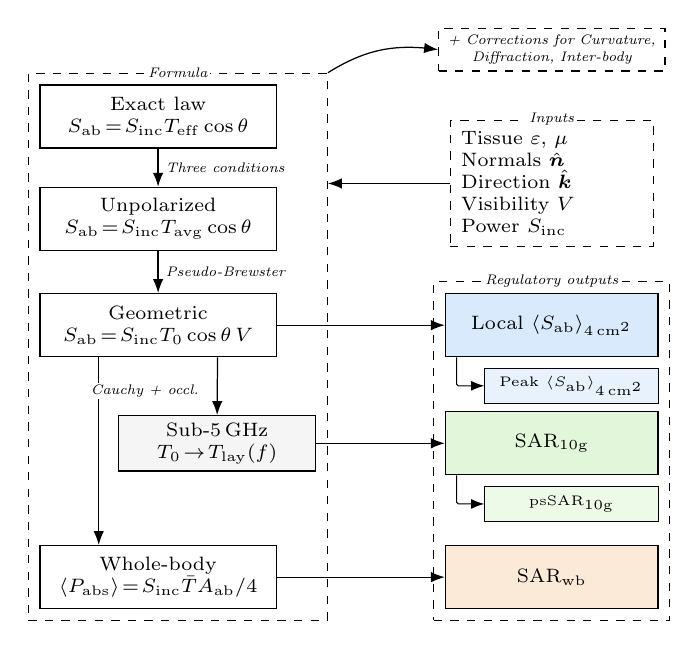
\begin{tikzpicture}[
    every node/.style={font=\scriptsize},
    box/.style={draw=black, line width=0.5pt, rectangle,
                inner sep=2pt, minimum height=8mm, minimum width=30mm,
                fill=white, align=center, font=\scriptsize},
    sub5/.style={draw=black, line width=0.5pt, rectangle,
                inner sep=2pt, minimum height=7mm, minimum width=25mm,
                fill=black!4, align=center, font=\scriptsize},
    outbox/.style={draw=black, line width=0.5pt, rectangle,
                inner sep=2pt, minimum height=8mm, minimum width=27mm,
                align=center, font=\scriptsize},
    smallout/.style={draw=black, line width=0.4pt, rectangle,
                inner sep=1.5pt, minimum height=4.5mm, minimum width=22mm,
                align=center, font=\tiny},
    inputs/.style={draw=black, line width=0.4pt, rectangle, dashed,
                inner sep=4pt, text width=23mm, align=left,
                font=\scriptsize, fill=white},
    corrbox/.style={draw=black, line width=0.4pt, rectangle, dashed,
                inner sep=2.5pt, text width=27mm, align=center,
                font=\tiny\itshape, fill=white},
    arrow/.style={->, line width=0.45pt, >=Latex},
    smallarrow/.style={->, line width=0.4pt, >=Latex,
                rounded corners=0.6pt},
    tag/.style={font=\tiny\itshape, align=center,
                fill=white, inner sep=0.6pt}
]
  % --- Spine: Exact -> Unpolarized -> Geometric -> Whole-body ---
  \node[box] (exact) at (1.5, 0)     {Exact law\\$\Sab\!=\!\Sinc T_{\mathrm{eff}}\cos\theta$};
  \node[box] (avg)   at (1.5, -1.30) {Unpolarized\\$\Sab\!=\!\Sinc \Tavg\cos\theta$};
  \node[box] (geom)  at (1.5, -2.65) {Geometric\\$\Sab\!=\!\Sinc T_0\cos\theta\,\Vis$};
  \node[box] (whole) at (1.5, -5.85) {Whole-body\\$\langle P_{\mathrm{abs}}\rangle\!=\!\Sinc\Tbar\Aab/4$};

  % --- Sub-5 GHz inside Formula ---
  \node[sub5] (layered) at (2.25, -4.15) {Sub-5\,GHz\\$T_0\!\to\!\Tlay(f)$};

  % --- Outputs (mains centered at x=6.5; smalls right-aligned) ---
  % Main width 27mm -> right edge at 7.85; small width 22mm centered
  % at x=6.75 has right edge 7.85 (right-aligned).
  \node[outbox, fill=outA] (outLocal) at (6.5, -2.65) {Local $\SabAvg$};
  \node[smallout, fill=outA!60] (outLocalPeak) at (6.75, -3.42) {Peak $\SabAvg$};

  \node[outbox, fill=outC] (outCube) at (6.5, -4.15) {$\mathrm{SAR}_{10\mathrm{g}}$};
  \node[smallout, fill=outC!60] (outCubePeak) at (6.75, -4.92) {$\mathrm{psSAR}_{10\mathrm{g}}$};

  \node[outbox, fill=outB] (outWB) at (6.5, -5.85) {$\mathrm{SAR}_{\mathrm{wb}}$};

  % --- Spine arrows top three ---
  \draw[arrow] (exact) -- node[tag,right=2pt] {Three conditions} (avg);
  \draw[arrow] (avg)   -- node[tag,right=2pt] {Pseudo-Brewster}   (geom);

  % --- Geom -> Whole at 1/4 width of both ---
  \coordinate (geom_q1) at ($(geom.south west)!0.25!(geom.south east)$);
  \coordinate (whole_q1) at ($(whole.north west)!0.25!(whole.north east)$);
  \draw[arrow] (geom_q1) -- node[tag,right=2pt,pos=0.18,xshift=-2mm] {Cauchy + occl.} (whole_q1);

  % --- Geom -> Sub-5 GHz at 3/4 width ---
  \coordinate (geom_q3) at ($(geom.south west)!0.75!(geom.south east)$);
  \draw[arrow] (geom_q3) -- (layered.north);

  % --- Horizontal east-west arrows from spine to outputs ---
  \draw[arrow] (geom.east)   -- (outLocal.west);
  \draw[arrow] (layered.east) -- (outCube.west);
  \draw[arrow] (whole.east)  -- (outWB.west);

  % --- |-> elbow arrows main.south_west -> small.west ---
  \draw[smallarrow] ($(outLocal.south west) + (1.5mm,0)$) |- (outLocalPeak.west);
  \draw[smallarrow] ($(outCube.south west)  + (1.5mm,0)$) |- (outCubePeak.west);

  % --- Formula and Outputs dashed groups ---
  \begin{pgfonlayer}{background}
    \node[draw=black, line width=0.4pt, dashed,
          fit=(exact)(whole)(layered),
          inner sep=4pt,
          name=formulabox,
          label={[font=\tiny\itshape, anchor=center, fill=white, inner sep=1pt]north:Formula}] {};
    \node[draw=black, line width=0.4pt, dashed,
          fit=(outLocal)(outLocalPeak)(outCube)(outCubePeak)(outWB),
          inner sep=4pt,
          label={[font=\tiny\itshape, anchor=center, fill=white, inner sep=1pt]north:Regulatory outputs}] {};
  \end{pgfonlayer}

  % --- Inputs box (lowered further) ---
  \node[inputs, label={[font=\tiny\itshape, anchor=center, fill=white, inner sep=1pt]north:Inputs}] (inp) at (6.5, -0.85) {%
    Tissue $\varepsilon$, $\mu$\\
    Normals $\nhat$\\
    Direction $\khat$\\
    Visibility $\Vis$\\
    Power $\Sinc$};

  % --- Inputs -> Formula: from middle of inp.west, horizontal,
  % ending at the right edge of the Formula dashed box.
  \draw[arrow] (inp.west) -- (formulabox.east |- inp);

  % --- Corrections small dashed box above the Inputs ---
  \node[corrbox] (corr) at (6.5, 0.85)
    {+ Corrections for Curvature,\\Diffraction, Inter-body};

  % --- Curved arrow from Formula box to Corrections box ---
  \draw[arrow] (formulabox.north east) to[bend left=20] (corr.west);
\end{tikzpicture}
\end{document}
